% Created 2016-12-20 Tue 18:34
% Intended LaTeX compiler: pdflatex
\documentclass[journal,onecolumn]{IEEEtran}
                            \usepackage[pdftex]{graphicx}
\graphicspath{{../pdf/}{../jpeg/}}
\DeclareGraphicsExtensions{.pdf,.jpeg,.png}
\usepackage[cmex10]{amsmath}
\interdisplaylinepenalty=2500
\usepackage{cite}
\usepackage{epsfig}
\usepackage{epstopdf}
\usepackage[caption=false,font=footnotesize]{subfig}
\usepackage{bm}
\usepackage{color}
\usepackage{hyperref}
\author{Author 1, Author 2}
\date{\today}
\title{Design and analysis of a soft continuum robot prototype for colonoscopy}
\hypersetup{
 pdfauthor={Author 1, Author 2},
 pdftitle={Design and analysis of a soft continuum robot prototype for colonoscopy},
 pdfkeywords={},
 pdfsubject={},
 pdfcreator={Emacs 24.5.1 (Org mode 9.0.1)}, 
 pdflang={English}}
\begin{document}

\maketitle
%\markboth{Journal of \LaTeX\ Class Files,~Vol.~6, No.~1, January~2007}%
%{Shell \MakeLowercase{\textit{et al.}}: Bare Demo of IEEEtran.cls for Journals}

%\IEEEpubid{0000--0000/00\$00.00~\copyright~2007 IEEE}

%\IEEEspecialpapernotice{(Invited Paper)}

%\maketitle

\begin{abstract}
%\boldmath
The abstract goes here.
\end{abstract}

\begin{IEEEkeywords}
IEEEtran, journal, \LaTeX, paper, template.
\end{IEEEkeywords}

\IEEEpeerreviewmaketitle


\section{Introduction}
\label{sec:orgf3c504f}
\begin{itemize}
\item 1st paragraph: To introduce the advantages of using soft robots in endoscopy
\begin{itemize}
\item Clinical data of endoscopy, showing the increasing need of robotic endoscope
\item Review of some state-of-the-art robot-assisted endoscopy with rigid structure
\begin{itemize}
\item tendon-driven
\end{itemize}
\item Current applications of soft robots in medical applications
\item Advantages of using soft robots in endoscopy
\begin{itemize}
\item low-cost 
\begin{itemize}
\item disposable
\end{itemize}
\item easy to fabricate
\item particularly fluidically-driven soft continuum robots
\end{itemize}
\end{itemize}

\item 2nd paragraph: To introduce the technical challenges of using soft robots in endoscopy
\begin{itemize}
\item State-of-the-art soft robotic technologies
\begin{itemize}
\item achievements in literature
\end{itemize}
\item requirements for endoscopy
\begin{itemize}
\item safe
\item fast response
\item small size
\item with working channel *
\item (with embedded camera)
\end{itemize}
\item the technical challenges in design:
\begin{itemize}
\item choice of material
\item structural and geometrical design
\item how stiff should be enough?
\item simulation of hyper-elastic materials and interaction with internal instrument
\end{itemize}
\end{itemize}

\item 3rd paragraph: How do we solve these challenges
\begin{itemize}
\item state-of-the-art FEA for hyperelastic material
\begin{itemize}
\item achievement in literature
\end{itemize}
\item what are the contributions of our FEA?
\begin{itemize}
\item any literature have done simulation of interaction with internal instrument?
\item 
\end{itemize}
\item what are our approach/tricks that can approximate the hyperelastic behaviour?
\begin{itemize}
\item new FEM formulations?
\item new combination of element?
\item optimized for fast computation?
\item etc\ldots{}
\end{itemize}

\item how the FEA results be incorporate in the design optimization
\begin{itemize}
\item description of role of FEA in the design optimization cycle
\end{itemize}

\item Fig. \ref{fig:orgfa82c82}. The endoscope prototype.

\begin{figure}[!h]
\centering
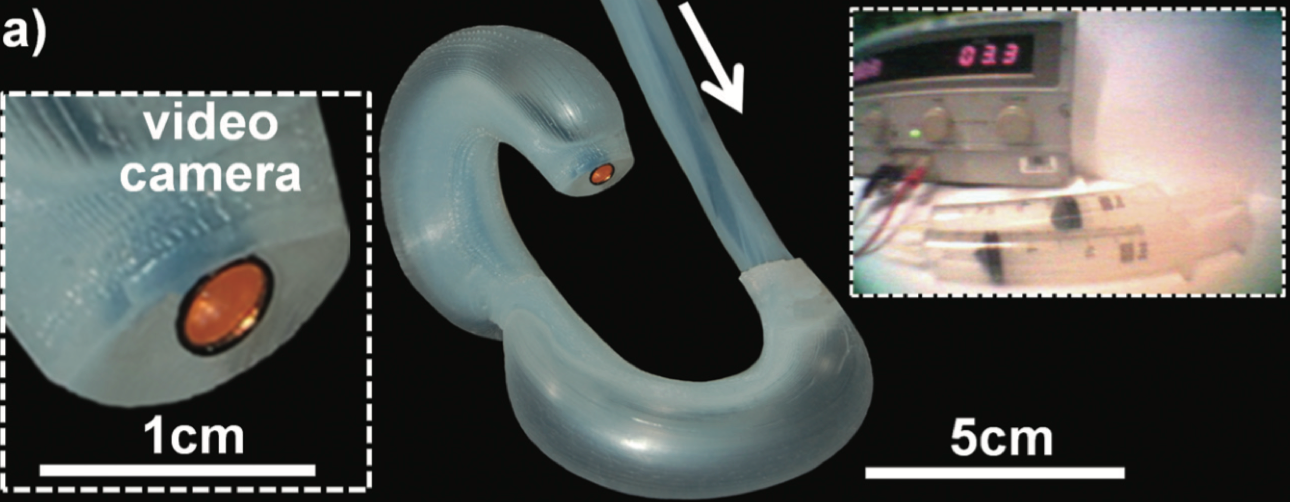
\includegraphics[width=0.6\textwidth]{./fig/fig-robot_intro.png}
\caption{\label{fig:orgfa82c82}
The endoscope prototype.}
\end{figure}

\item 4rd paragraph: Clearly list out the contributions using the proposed FEM-based design 
\begin{enumerate}
\item Novel structural design to improve the stiffness and durability (section \ref{sec:org7104326})
\begin{itemize}
\item dump-bell-shaped actuation chamber
\end{itemize}
\item FEM methods for simulating the effects of including working channel (section \ref{sec:orgcb620bb})
\begin{itemize}
\item e.g. buckling
\end{itemize}
\item The smallest soft continuum robot with working channel (øxmm) for endoscopic interventions (section \ref{sec:org21b22ba})
\begin{itemize}
\item how much output force?
\item smallest too aggressive?
\end{itemize}
\end{enumerate}
\end{itemize}
\end{itemize}


\section{Materials and methods}
\label{sec:org5257bcd}


\subsection{Design and performance requirements}
\label{sec:org12c4c04}
\begin{itemize}
\item specify the target application -- colonoscopy

\item a working channel is preserved
\begin{itemize}
\item for biopsy, suction, irrigation, and other instruments
\item give common dimension of clinically-used instruments (e.g. biopsy forceps)
\begin{itemize}
\item dimensions in specific applications: e.g. colonoscopy
\end{itemize}
\item requirement for the diameter: the larger the better
\begin{itemize}
\item specify a dimension for the prototype in this paper
\end{itemize}
\end{itemize}

\item target dimension: Outer diameter and length
\begin{itemize}
\item why such dimension?
\begin{itemize}
\item clinical reason
\end{itemize}
\end{itemize}

\item The requirement of bending behavior
\begin{itemize}
\item curvature ratio
\item 
\end{itemize}

\item constrained elongation
\begin{itemize}
\item i.e. only bending without much elongation
\item why?
\begin{itemize}
\item camera is mount at the tip. bending with large elongation will cause loss of tracked vision target in the endoscopic view
\end{itemize}
\end{itemize}

\item How stiff should the scope be? - the key problem of this paper
\begin{itemize}
\item sufficient to be stable during instrument manipulation
\item sufficient to withstand high input pressure
\item we use FEM simulations to characterize the stiffness properties
\end{itemize}

\item Durability
\begin{itemize}
\item long life cycle
\end{itemize}

\item actuation method - fluidic actuation 
\begin{itemize}
\item advantages of fluidically driven - can be only Hydraulic/pneumatic
\begin{itemize}
\item safe without internal electric component or some toxic component
\item hydraulic: incompressible transmission media gives fast response, \ldots{}
\item pneumatic: ease of assembly, \ldots{}
\item MRI-compatible
\item a sentence about the control method
\item why not tendon-driven? (move to discussion section)?
\begin{itemize}
\item here we may need to mention also the advantages of tendon-driven soft continuum robot
\end{itemize}
\end{itemize}
\end{itemize}

\item discuss difficulties of miniaturization - the inclusion of working channel
\begin{itemize}
\item mention the state-of-the-art (smallest) soft robot dimension (for colonoscopy)
\item difficulties of including a central working channel
\begin{itemize}
\item weaken structure
\item reduced volume of material --> less elongation and thus smaller bending curvature
\end{itemize}
\item are we the first soft robot with working channel of that small dimension?
\end{itemize}

\item Assume that the camera and LED are not considered during simulation, but they are included in the real prototype.
\end{itemize}


\subsection{Structural design}
\label{sec:org7104326}
\begin{itemize}
\item the actuation response depends on the structural design
\begin{itemize}
\item the geometric design of the actuation chambers and internal tubings
\item materials
\item fabrication process
\end{itemize}
\item we use FEA to simulate the kinematic and dynamics behaviour in the design optimization process, regarding to the first two factors

\item we can first give the design using fan-shaped actuation chambers
\item then use FEM to demonstrate the weak points at the chamber corners
\item then provide the dump-bell-shaped design
\end{itemize}

\subsubsection{Geometrical design of actuation chambers}
\label{sec:org1aad666}

\begin{itemize}
\item Fig. \ref{fig:org0f1c4a7}. 2D FEM model

\begin{figure}[!h]
\centering
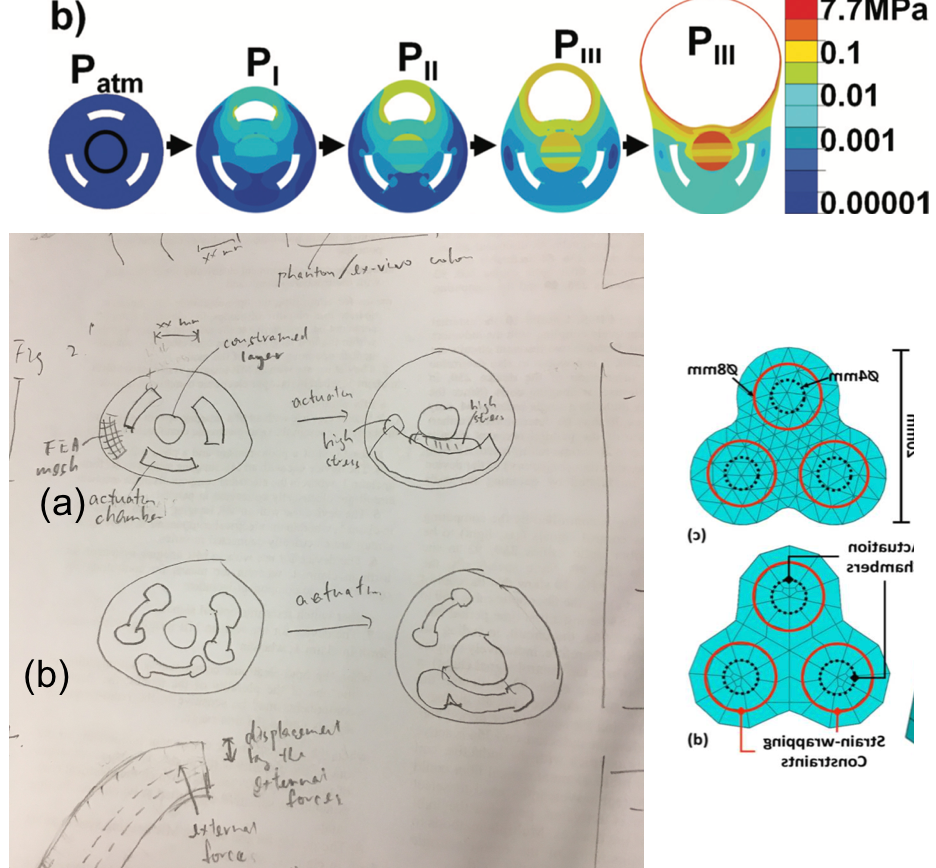
\includegraphics[width=0.6\textwidth]{./fig/fig-2D_fem.png}
\caption{\label{fig:org0f1c4a7}
Internal stress during actuation. (a) Fan-shaped actuation chamber design has higher stress. (b) Dump-bell shaped chamber design has lower stress.}
\end{figure}
\end{itemize}


\begin{itemize}
\item actuation chamber design - 1st version: the fan-shaped 
\begin{itemize}
\item number of chambers
\begin{itemize}
\item 3-chambers are commonly used in the literature
\end{itemize}
\item chamber geometry
\begin{itemize}
\item why do we use the fan-shaped chamber?
\item done in~\cite{martinez2012robotic}.
\end{itemize}
\item mention about chamber arrangement/location
\begin{itemize}
\item why this offset from the center?
\end{itemize}
\end{itemize}
\item constraint layers
\begin{itemize}
\item where are the constraint layers
\item what are the benefits of the constraint layers?
\item why they are necessary?
\end{itemize}
\item dimension of the working channel
\begin{itemize}
\item to match requirement mention in \ref{sec:org12c4c04}
\end{itemize}

\item actuation chamber design - 2nd version: the dump-bell shaped
\begin{itemize}
\item thicker walls between the chambers and the central channel
\item no-corner chambers
\item why?
\begin{itemize}
\item during actuation, high stress are found in the fan-shaped chambers 
\begin{itemize}
\item in the walls between the chambers and the central channel
\item at the corners
\end{itemize}
\end{itemize}
\end{itemize}
\end{itemize}


\subsubsection{The choice of materials}
\label{sec:org9591329}

\begin{itemize}
\item Fig. \ref{fig:orge39dc7f}. Stress-strain characteristics of the materials in used 

\begin{figure}[!h]
\centering
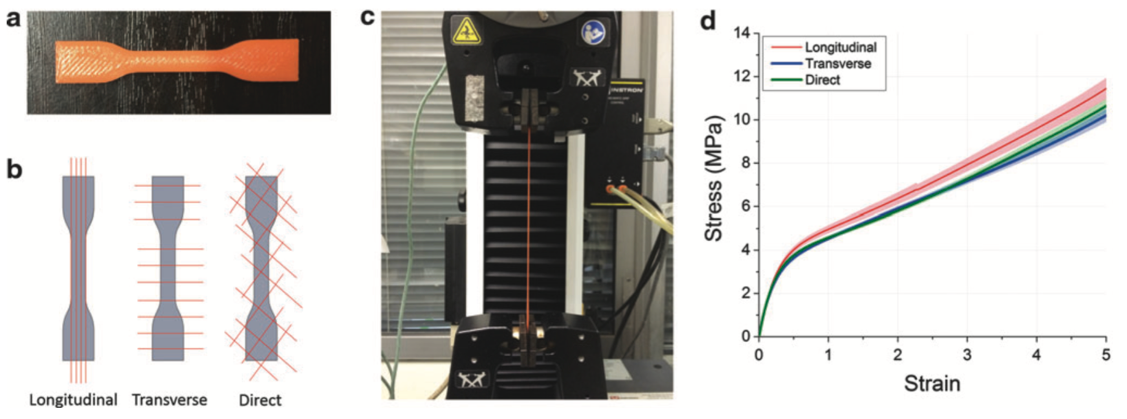
\includegraphics[width=0.6\textwidth]{./fig/fig-stress_strain_material.png}
\caption{\label{fig:orge39dc7f}
Stress-strain curves of the materials in used. These measurement data are used for identification of hyperelastic model in Table \ref{tab:org95e34f9}.}
\end{figure}
\end{itemize}


\begin{itemize}
\item show the stress-strain properties of the material (Fig. \ref{fig:orge39dc7f})
\begin{itemize}
\item the body
\begin{itemize}
\item the constraint layer
\item the central channel
\item both longitudinal and axial stress-strain
\item show failure limit
\end{itemize}
\end{itemize}
\item reasons for the choice
\begin{itemize}
\item for the body
\begin{itemize}
\item large longitudinal strain
\item can withstand high stress
\end{itemize}
\item for the constraint layer
\begin{itemize}
\item insignificant axial strain
\item can withstand high stress
\end{itemize}
\item for the central channel
\begin{itemize}
\item insignificant axial strain
\item can withstand high stress
\end{itemize}
\end{itemize}
\end{itemize}

\subsection{FEM-based modeling and response characterization}
\label{sec:orgcb620bb}

\subsubsection{Identification of hyperelastic model}
\label{sec:org91f42dd}
\begin{itemize}
\item Table \ref{tab:org95e34f9}. Table of hyperelastic models

\begin{table}[!p]
\caption{\label{tab:org95e34f9}
Hyperelastic model candidates for FEM simulation.}
\centering
\begin{tabular}{p{0.8\textwidth}}
\begin{center}
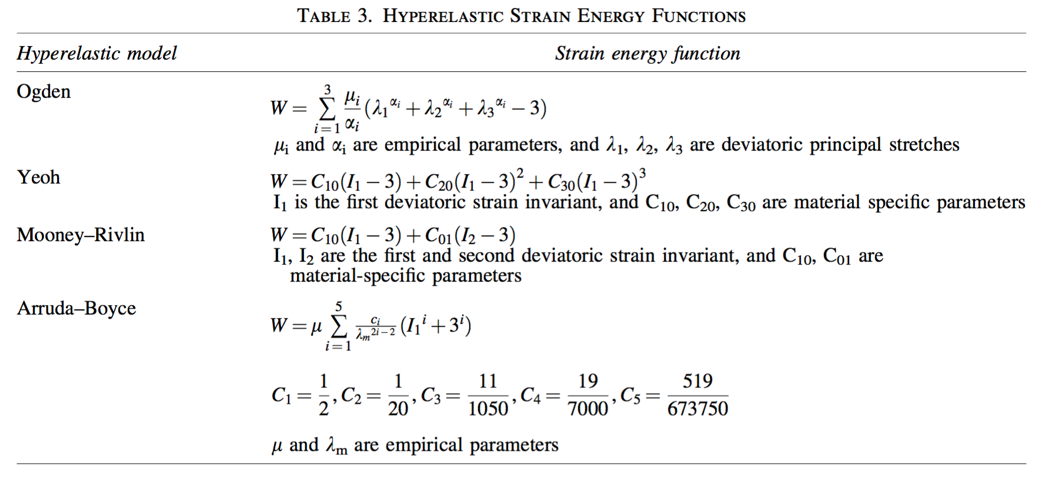
\includegraphics[width=.9\linewidth]{./fig/tab1.png}
\end{center}\\
\end{tabular}
\end{table}

\item Table \ref{tab:org0f1e665}. FEM simulation parameters

\begin{table}[!p]
\caption{\label{tab:org0f1e665}
FEM simulation parameters.}
\centering
\begin{tabular}{p{0.8\textwidth}}
\begin{center}
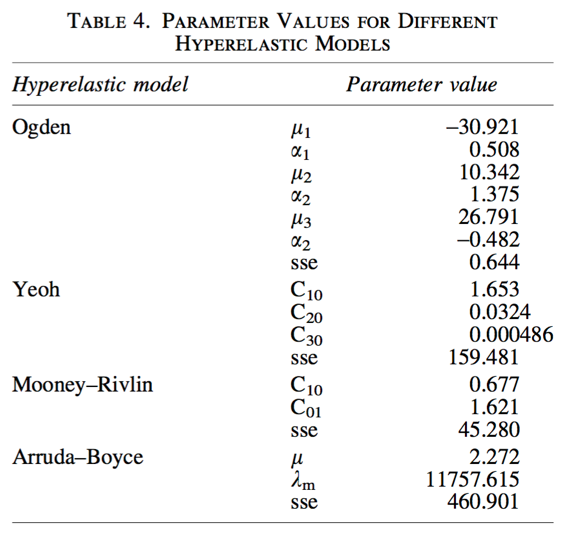
\includegraphics[width=.9\linewidth]{./fig/tab2.png}
\end{center}\\
\end{tabular}
\end{table}
\end{itemize}


\begin{itemize}
\item the identifying hyperelastic materials for FEA
\begin{itemize}
\item how to choose the strain energy functions?
\begin{itemize}
\item list several candidates, and then discuss how to choose among them.
\end{itemize}
\item what software you are using?
\end{itemize}

\item how to choose the finite element? and why?
\begin{itemize}
\item hexahedral element for the hyperelastic material, truss for the constraint layer?
\begin{itemize}
\item with the element number in that software (e.g. Abaqus element type C3D10H)
\end{itemize}
\end{itemize}

\item Simulation parameters
\begin{itemize}
\item what is the number of elements?
\item what are the types of elements?
\item simulation time
\item list in a table
\end{itemize}
\end{itemize}


\subsubsection{Characterization of bending behavior and stiffness}
\label{sec:orge3e943e}

\begin{itemize}
\item Fig. \ref{fig:org62ae81e}. 3D FEM model for stiffness simulation

\begin{figure}[!h]
\centering
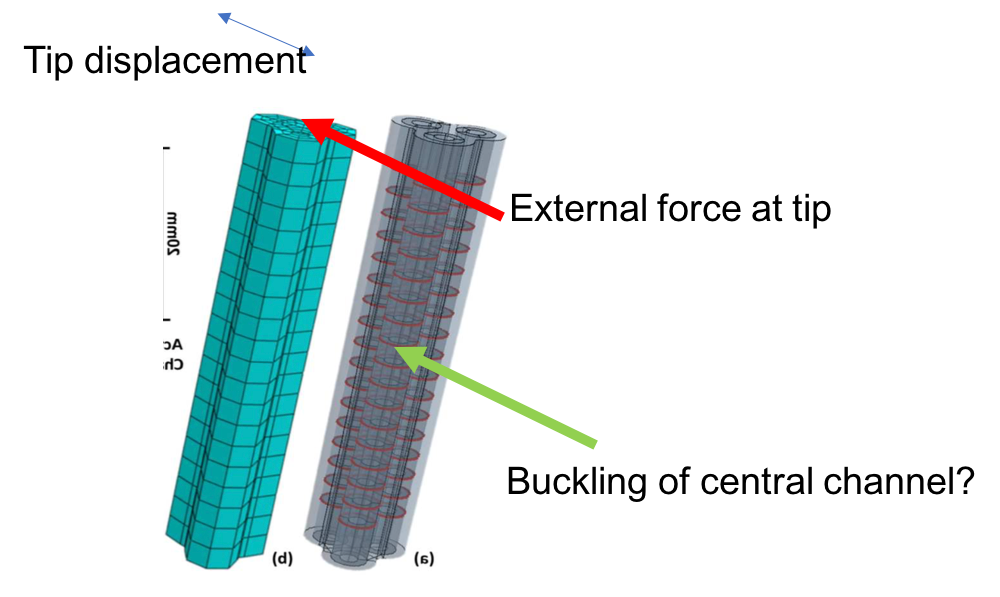
\includegraphics[width=0.6\textwidth]{./fig/fig-FEA_3D_external_tipforce.png}
\caption{\label{fig:org62ae81e}
FEM simulation to estimate the robot stiffness. An external force is exerted at the tip perpendicular to the pointing direction. Stiffer robot requires larger force to move the tip.}
\end{figure}
\end{itemize}



\begin{itemize}
\item simulate bending performance: ratio = curvature/length
\item bending force 
\begin{itemize}
\item what is bending force? the force at the tip ?
\item the force with the same direction with the tip movement
\end{itemize}
\end{itemize}


\begin{itemize}
\item how to estimate stiffness?
\begin{itemize}
\item applying a force to the inner wall of the working channel
\item stiffness = force / displacement
\end{itemize}
\end{itemize}


\begin{itemize}
\item we need to simulate the stress acting on the embedded tubings?
\begin{itemize}
\item can we simulate the buckling of the tubing? when and how the buckling occurs?
\item as including a central channel is also the key difference from the literature, such simulation will be the novelty of the method
\item buckling causes collapse and thus malfunction of the central channel.
\end{itemize}
\end{itemize}


\subsection{(Fabrication process) - optional}
\label{sec:org2992447}

\begin{itemize}
\item Fig. \ref{fig:org65c33a6}. Fabrication procedure -- optional

\begin{figure}[!h]
\centering
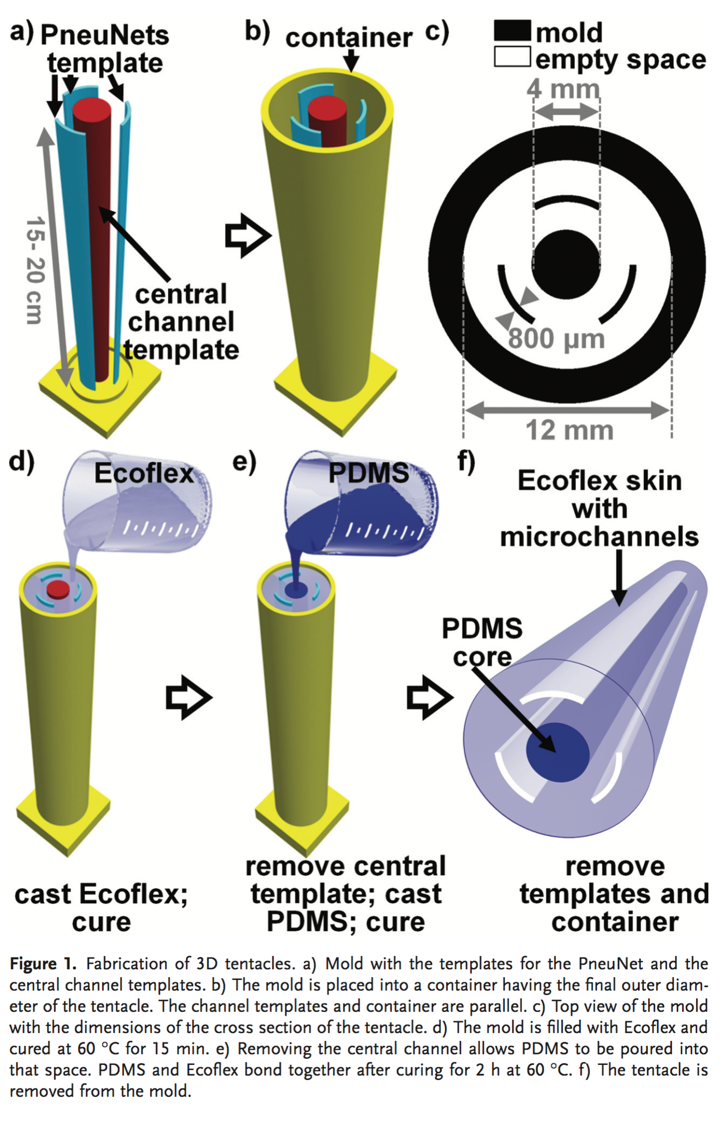
\includegraphics[width=0.6\textwidth]{./fig/fig-fabrication.png}
\caption{\label{fig:org65c33a6}
Fabrication procedure of the endoscope prototype. - optional}
\end{figure}

\item Fabrication process
\begin{itemize}
\item low-cost
\item basic procedure (of course some basic tricks that can be disclosed)
\begin{itemize}
\item e.g. sequence of molding and filling material, temperature
\item reference: e.g.  Fig.1 in ~\cite{martinez2012robotic}.
\end{itemize}
\item what should be paid attention to? why?
\begin{itemize}
\item e.g. temperature control, material filling speed, assembly cautions
\item \ldots{}
\end{itemize}
\end{itemize}
\end{itemize}


\section{Results and discussion}
\label{sec:org21b22ba}
\begin{itemize}
\item Comparison of the results between FEA and the real robot

\item workspace analysis
\begin{itemize}
\item using random pressure inputs
\end{itemize}
\item how to measure the bending force
\item how to measure the internal force
\begin{itemize}
\item fatigue test
\begin{itemize}
\item no. of cycle until failure
\end{itemize}
\item can take reference from \href{file:///Users/Denny/paper_lib/High-Force Soft Printable Pneumatics for Soft Robotic Applications.pdf}{yap2016highforce}
\end{itemize}
\end{itemize}

\subsection{Quasi-static bending behavior}
\label{sec:org904213d}

\begin{itemize}
\item Fig \ref{fig:orgbab9cca}. Bending behaviour 

\begin{figure}[!h]
\centering
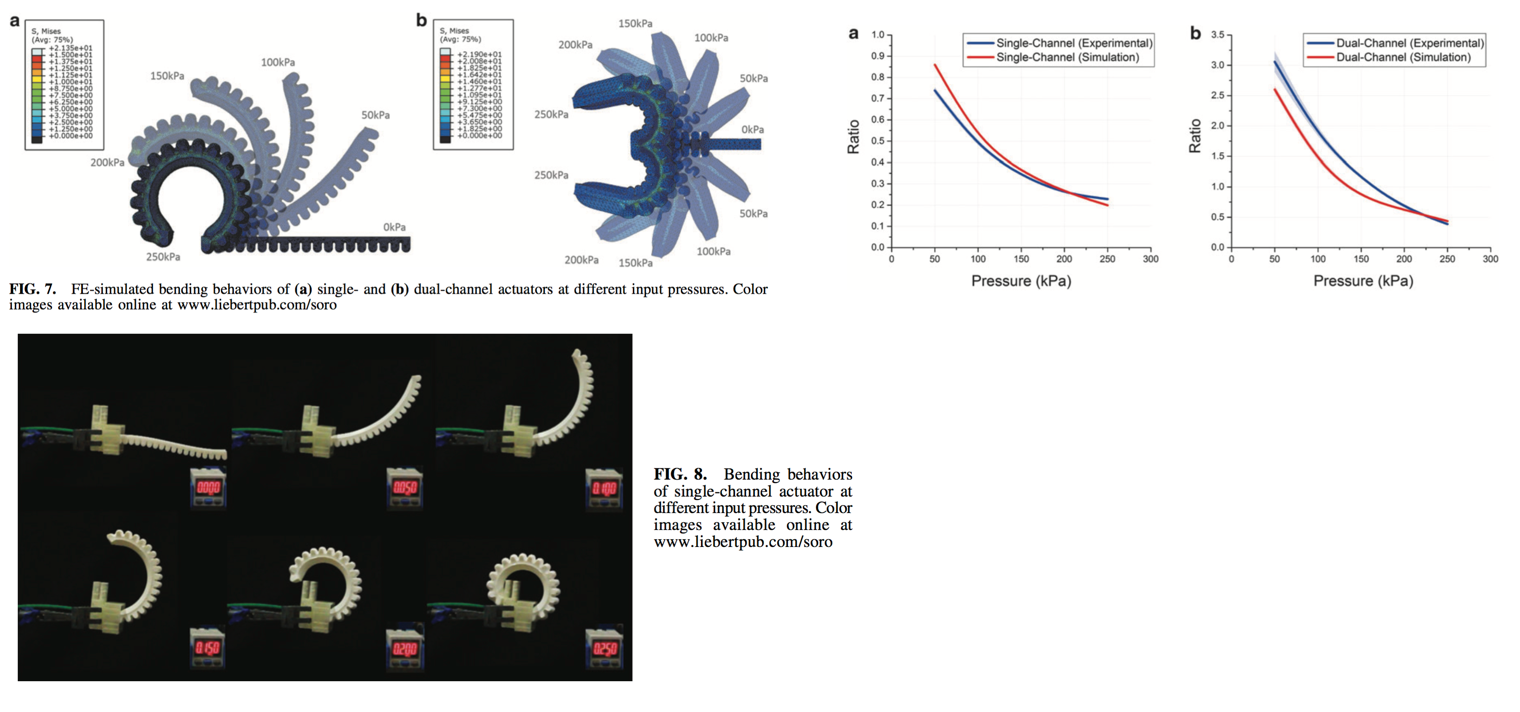
\includegraphics[width=0.6\textwidth]{./fig/fig-bending_behavior.png}
\caption{\label{fig:orgbab9cca}
Bending behavior of the endoscope. (a) FEA results with different chamber pressure. (b) Snapshots of the real robot. (c) The relationship between chamber pressure and the bending curvature, for different preloaded pressure. (d) Bending coplanarity of the prototype. (e) Workspace of the prototype.}
\end{figure}

\item experiment settings
\begin{itemize}
\item the prototype based is fixed
\begin{itemize}
\item what were measured?
\begin{itemize}
\item bending radius
\item length of the prototype
\item position of the tip
\end{itemize}
\item what instruments were used?
\begin{itemize}
\item e.g. EM tracker to measure the 3D position of the tip
\item e.g. analyzed from captured images to measure the radius and the length
\end{itemize}
\end{itemize}
\item actuation condition?
\begin{itemize}
\item bending when actuating 1 chamber
\item bending when actuating 2 chambers
\item different preloaded pressure
\item 
\end{itemize}
\item refer a figure that can illustrate the setting
\end{itemize}
\end{itemize}


\begin{itemize}
\item Assessment of the bending degree
\begin{itemize}
\item ratio = bending radius/length
\item lower ratio means better bending degree
\item both FEA and real robot results
\item real robot data of different preloaded pressure
\item 2 figures:
\begin{enumerate}
\item ratio vs chamber pressure
\item length vs chamber pressure
\end{enumerate}
\item expected results
\begin{itemize}
\item 
\end{itemize}
\end{itemize}

\item workspace analysis
\begin{itemize}
\item real robot data is enough
\item actuation of 1 and 2 chamber
\begin{itemize}
\item using random chamber pressure
\item uniform distribution
\end{itemize}
\item 1 result figure
\begin{itemize}
\item a 3D surface plot of the tip position
\item with some vectors showing the tip directions when adding more pressure at the 3 chambers
\end{itemize}
\item to show if the resulting cloud points are evenly distributed
\begin{itemize}
\item if the relationship of bending vs pressure is linear, the cloud points should be evenly distributed
\end{itemize}
\item expected results
\begin{itemize}
\item 
\end{itemize}
\end{itemize}
\end{itemize}


\begin{itemize}
\item (Assessment of motion coplanarity - optional)
\begin{itemize}
\item to examine if the bending is in a fixed plane
\item FEA may not reveal the coplanarity, because this might be due to some technical problems in the fabrication process, such as uneven material density
\item how to quantitatively measure the coplanarity?
\begin{itemize}
\item for each bending from 0 to max degree
\item obtain instantaneous velocities \(\{\bm{v}^{tip}\}_{k}\) of the tip at time step \(k\).
\begin{itemize}
\item \(k=0,...,N\) indicates the time step
\item let \(\bm{n}_{\theat}\) be the normal vector of the bending plane
\begin{itemize}
\item \(0\geq\theta\geq 2\pi\)
\end{itemize}
\item kinematics of the tip can be obtained using EM tracker
\end{itemize}
\item a scalar performance index evaluates if two consecutive velocities \(\bm{v}^{tip}_{i}\) and \(\bm{v}^{tip}_{i+1}\) stay on the bending plane
\begin{itemize}
\item \(J = (\bm{v}^{tip}_{i} \times \bm{v}^{tip}_{(i+1)}) \cdot \bm{n}_{\theta}\)
\end{itemize}
\item index closer to 0 means more coplanar bending
\end{itemize}
\item figures
\begin{itemize}
\item a 3D plot of the velocity vectors of a bending movement
\item showing the mean and the range of the coplanarity performance index of all recorded bending movements
\end{itemize}
\end{itemize}
\end{itemize}


\subsection{Stiffness analysis}
\label{sec:orgf8f8743}
\begin{itemize}
\item Fig. \ref{fig:orgfa879b2}. Stiffness measurement setting.

\begin{figure}[!h]
\centering
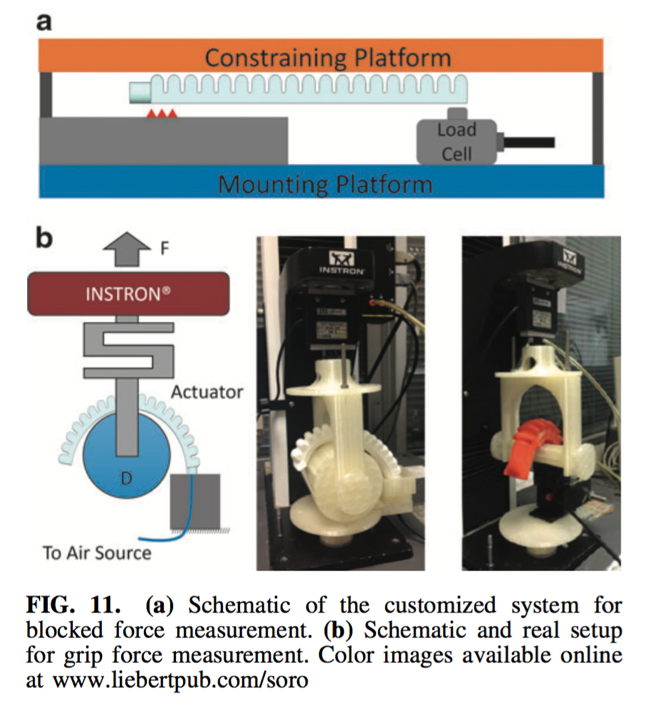
\includegraphics[width=0.6\textwidth]{./fig/fig-stiffness_test_setting.png}
\caption{\label{fig:orgfa879b2}
Stiffness measurement setting. The tip of the robot is connected to a pulling device with a force sensor. The robot is fixed to a platform. The platform is tilted to ensure the force is exerted perpendicular to the pointing direction.}
\end{figure}

\item Fig. \ref{fig:orgd6e64ad}. Stiffness results

\begin{figure}[!h]
\centering
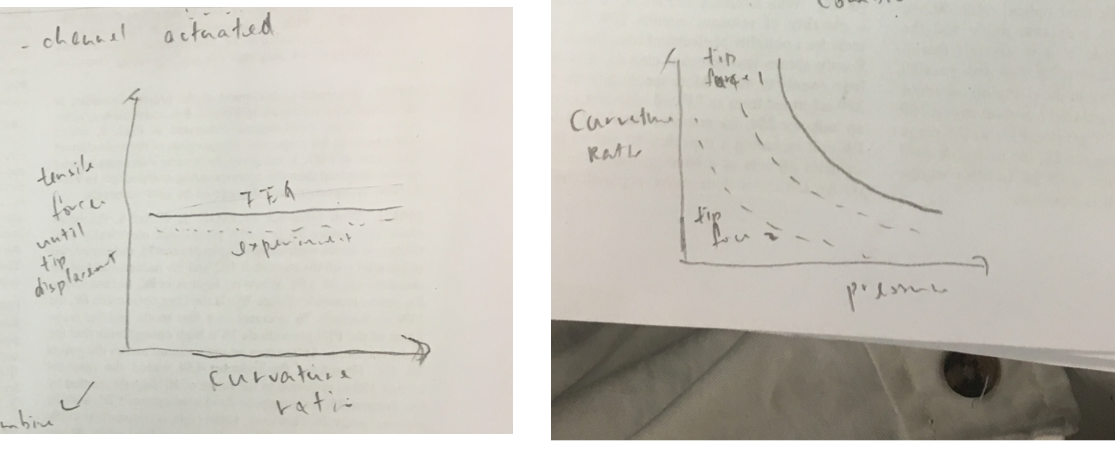
\includegraphics[width=0.6\textwidth]{./fig/fig-stiffness_results.png}
\caption{\label{fig:orgd6e64ad}
Stiffness of the protoype. (a) The min. force required to move the tip for Xmm vs curvature ratio, for different preloaded pressure. This force indicates the stiffness of the prototype. (b) The maximum displacement of the tip when accelerating a biopsy forceps inserted in the central channel.}
\end{figure}

\item experiment settings
\begin{itemize}
\item fig of the setting
\begin{itemize}
\item the robot base is fixed on a robotic platform
\item the tip of the robot is pulled by an external force
\begin{itemize}
\item pull until the tip is displaced (e.g. several mm)
\end{itemize}
\item the platform is tilted to ensure the pulling force acts perpendicularly to the robot pointing direction
\item the test is repeated with different robot bending angle
\end{itemize}
\item how to measure the force?
\begin{itemize}
\item type and name of the sensors
\end{itemize}
\item how to measure the displacement?
\begin{itemize}
\item EM tracking system?
\item Image analysis system?
\end{itemize}
\item conditions
\begin{itemize}
\item actuation of 1 chamber
\item actuation of 2 chambers
\item different preloaded pressure
\item 
\end{itemize}
\end{itemize}
\end{itemize}


\begin{itemize}
\item stiffer robot requires larger forces to displace the tip
\item Assessment of the stiffness - ratio: \(\frac{\textrm{pulling force}}{\textrm{tip displacement}}\)
\begin{enumerate}
\item min. force required to move the tip
\item displacement of the tip when accelerating a biopsy forceps (or a catheter) inserted in the central channel
\end{enumerate}
\item 2 result figures
\begin{enumerate}
\item force vs preloaded pressure
\begin{itemize}
\item several curves for different chamber pressure
\end{itemize}
\item displacement of the tip vs acceleration of the inserted instrument
\end{enumerate}
\item expected results
\begin{itemize}
\item for 1)
\begin{itemize}
\item larger force will be required when larger pressure is preloaded
\item at the same prelaoded pressure but with different chamber pressure, the values of the force required would be similar. Since a chamber pressure = a curvature ratio, we will similar stiffness for various curvature ratio.
\end{itemize}
\item for 2)
\begin{itemize}
\item Two increasing slopes will be observed.
\item more gentle slope before a certain value of the acceleration, the tip displacement will be insignificant.
\item A steeper slope after the value of acceleration.
\end{itemize}
\end{itemize}
\end{itemize}



\subsection{Dynamic response}
\label{sec:org48a5000}
\begin{itemize}
\item Fig. \ref{fig:orgecf1a7b}. Dynamic responses

\begin{figure}[!h]
\centering
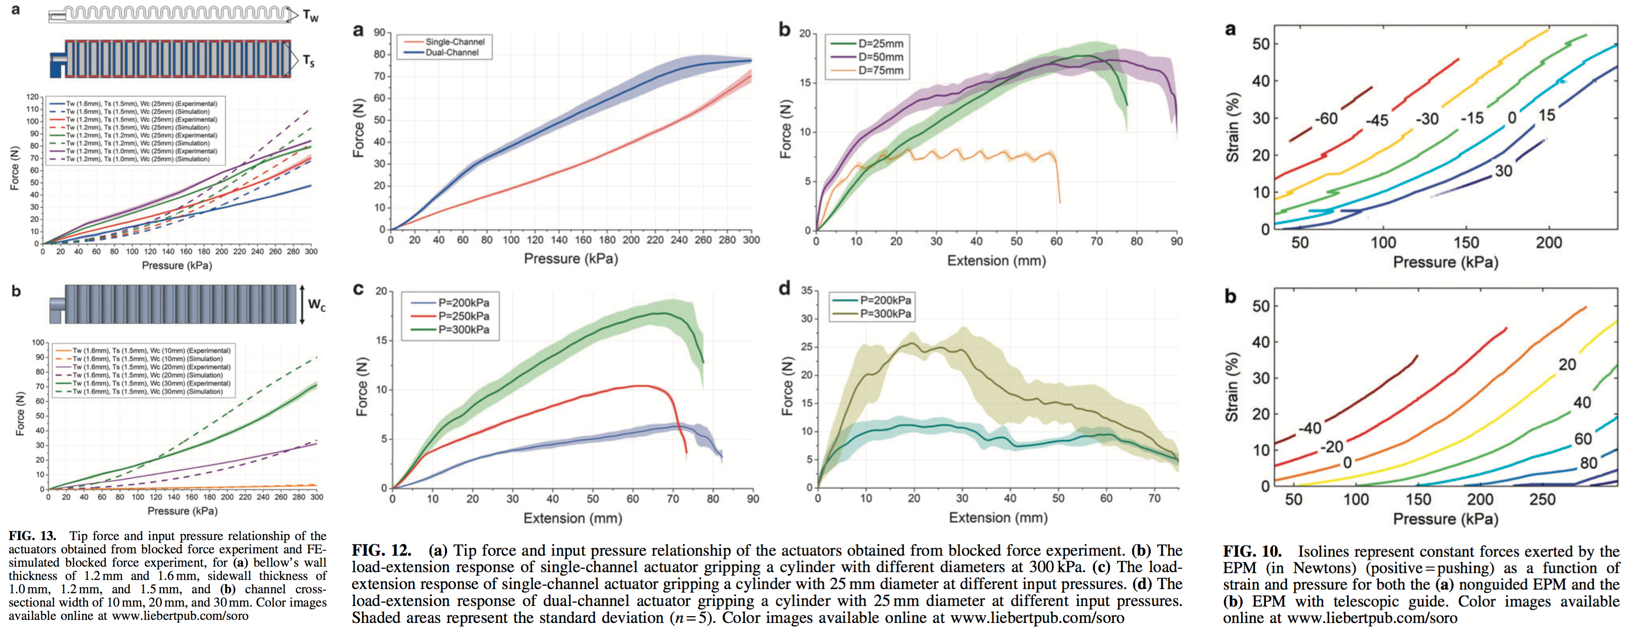
\includegraphics[width=0.6\textwidth]{./fig/fig-dynamic_response.png}
\caption{\label{fig:orgecf1a7b}
Dynamic response analysis. (a) The relationship of the tip force output and chamber pressure, for different preloaded pressure . (The tip force is measured while constraining the robot at 0 bending angle) Kinematics histories of the (b) step responses and (c) frequency responses of the robot.}
\end{figure}

\item experiment settings
\begin{enumerate}
\item for step response and frequency response:
\begin{itemize}
\item the same setting as the bending test in section \ref{sec:org904213d}
\item giving step input and sine input for the chamber pressure instead
\end{itemize}
\item for tip force output
\begin{itemize}
\item the same setting as the stiffness test in section \ref{sec:orgf8f8743}
\item not pull the tip, but giving pressure to the robot instead
\item measure the force at the tip
\item the force is perpendicular to the tip's pointing direction
\end{itemize}
\end{enumerate}
\item actuation condition
\begin{itemize}
\item 1 chamber actuation
\item 2 chambers actuation
\item different preloaded pressure
\item 
\end{itemize}
\item assessment of the dynamic response
\begin{enumerate}
\item tip force output
\item step response - typical performance indexes
\begin{itemize}
\item e.g. rise time
\item e.g. transient response
\item e.g. overshoot
\end{itemize}
\item frequency response - typical performance indexes
\begin{itemize}
\item frequency response plots
\end{itemize}
\end{enumerate}
\item result figures
\begin{enumerate}
\item tip force vs preloaded pressure
\begin{itemize}
\item several curves for different chamber pressure (i.e. curvature ratio)
\end{itemize}
\item time history of the tip displacement
\begin{itemize}
\item several curves for different preloaded pressure (i.e. curvature ratio)
\end{itemize}
\item frequency response plots
\begin{itemize}
\item amplitude vs frequency
\item phase vs frequency
\end{itemize}
\end{enumerate}
\item expected results
\begin{itemize}
\item 
\end{itemize}
\end{itemize}
\subsection{Performance Limits}
\label{sec:org26c3451}
\begin{itemize}
\item Fig. \ref{fig:orgdb518ec}. Prototype limits

\begin{figure}[!h]
\centering
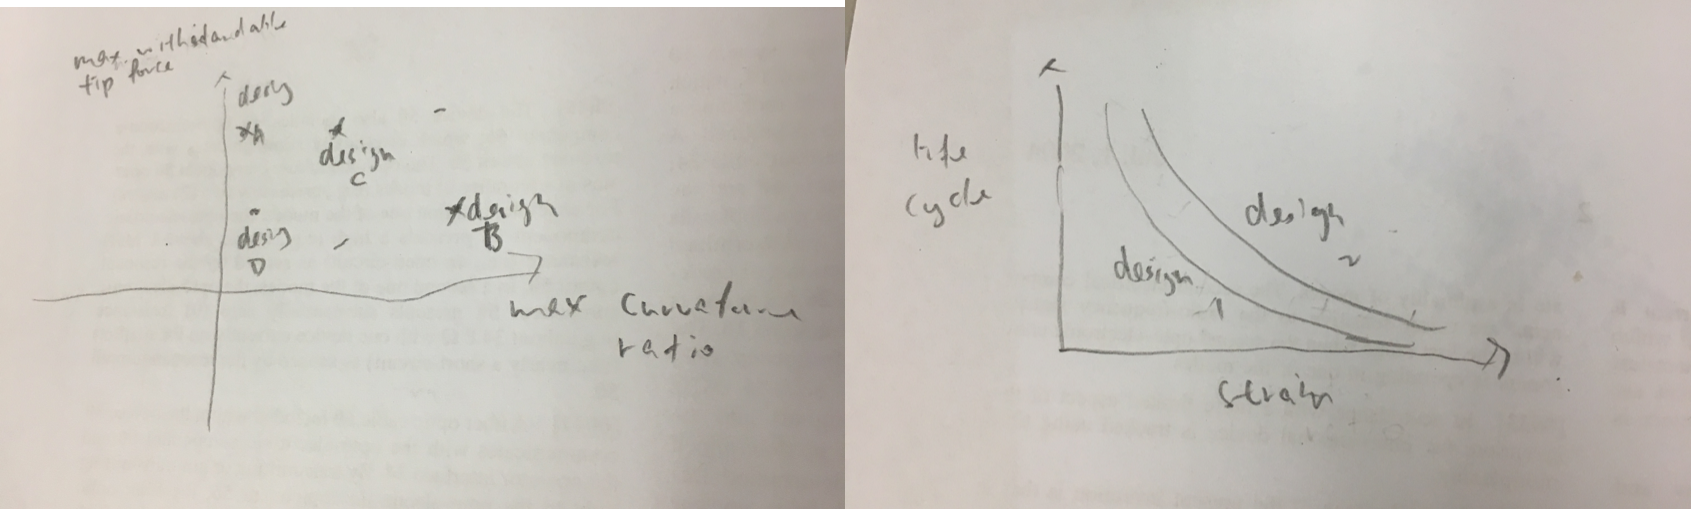
\includegraphics[width=0.6\textwidth]{./fig/fig-limits.png}
\caption{\label{fig:orgdb518ec}
Performance limits of the prototype for different preloaded pressure . (a) Stiffness vs max. curvature ratio. (b) Life cycle.}
\end{figure}

\item experiment settings
\begin{itemize}
\item increase the chamber pressure up to the maximum bending angle
\item measure the boundary curvature ratio
\item measure the tip force output
\item measure the life cycle
\end{itemize}
\item condition
\begin{itemize}
\item actuation of 1 chamber
\item actuation of 2 chambers
\item different preloaded pressure
\item 

\item run until failure
\end{itemize}

\item Assessment of the performance limits
\begin{enumerate}
\item The maximum curvature achieved
\begin{itemize}
\item curvature ratio of different preloaded pressure
\item can reuse/interpret the data obtained in the bending experiment in section \ref{sec:org904213d}
\item 
\end{itemize}
\item The maximum stiffness achieved
\begin{itemize}
\item define stiffness index = ratio: \(\frac{\textrm{pulling force}}{\textrm{tip displacement}}\)
\item stiffness of different preloaded pressure
\item can reuse/interpret the data obtained in the bending experiment in section \ref{sec:orgf8f8743}
\item 
\end{itemize}
\item life cycle 
\begin{itemize}
\item life cycle for different preloaded pressure
\begin{itemize}
\item 2 chamber actuated
\end{itemize}
\end{itemize}
\end{enumerate}
\item result figures
\begin{enumerate}
\item max. curvature ratio vs max. stiffness
\begin{itemize}
\item each point represents the value of a specific preloaded pressure
\end{itemize}
\item life cycle
\begin{itemize}
\item life cycle vs curvature ratio (\textasciitilde{}strain)
\begin{itemize}
\item several curves for different preloaded pressure
\end{itemize}
\end{itemize}
\end{enumerate}
\item expected results
\begin{itemize}
\item for 1) lower preloaded pressure will have lower stiffness and curvature ratio
\item for 2) using lower pressure will have longer life
\end{itemize}
\end{itemize}


\subsection{Discussion}
\label{sec:org1055a02}

\begin{itemize}
\item Fig. \ref{fig:orgbb5ed76}. Demonstration of basic endoscopic procedure

\begin{figure}[!h]
\centering
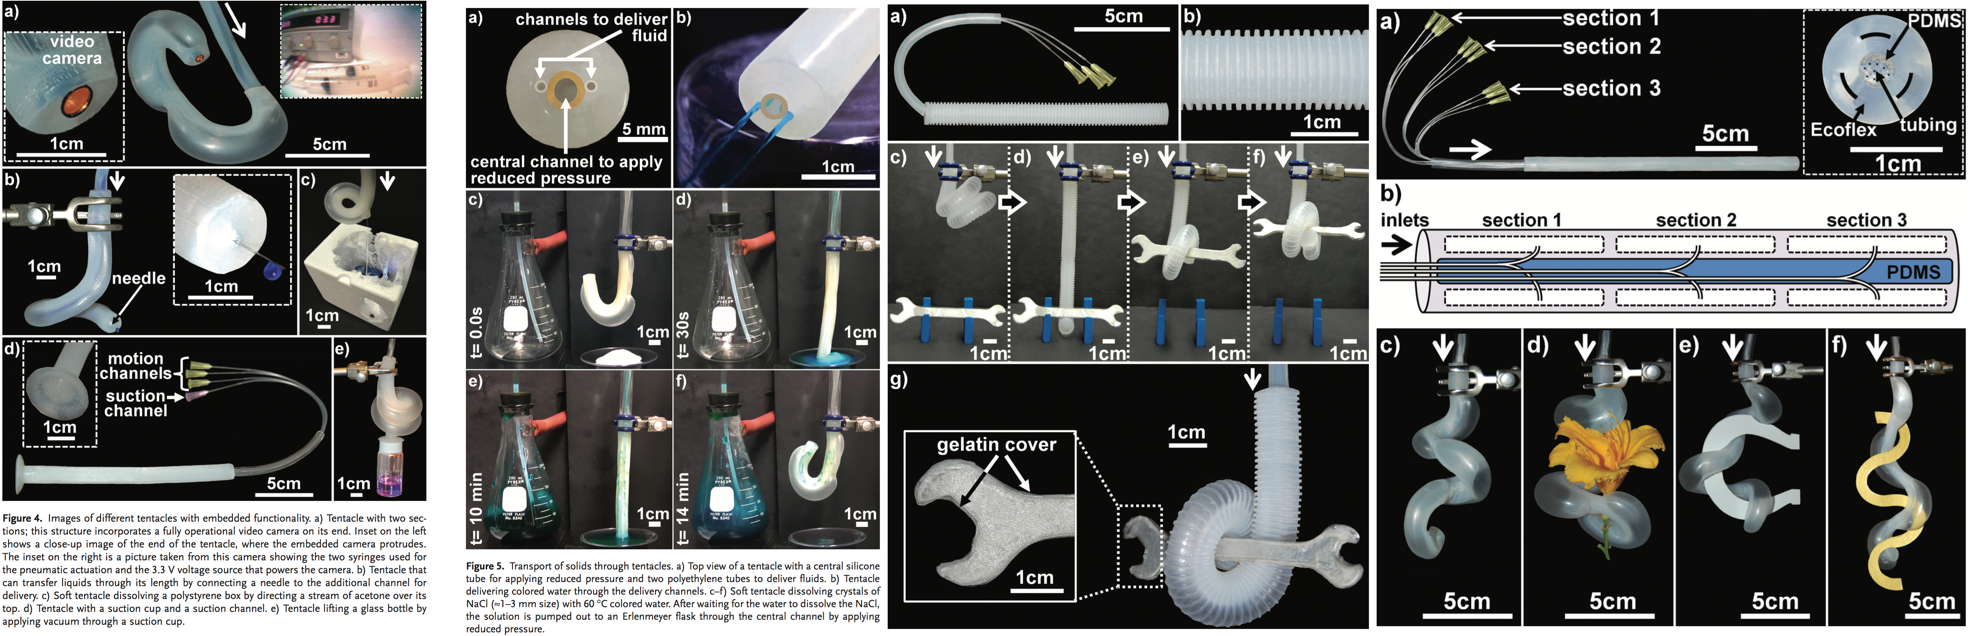
\includegraphics[width=0.6\textwidth]{./fig/fig-demo_basics.png}
\caption{\label{fig:orgbb5ed76}
Basic functions of the prototype. (a) Endoscopic view when performing a biopsy task inside a phantom model. (b) Suction and (c) Irrigation of colored liquid. The demonstrations can also be found in the provided videos.}
\end{figure}

\item Demonstrate the robot can perform basic functions for endoscopy
\begin{itemize}
\item endoscopic view
\item the use of working channel
\begin{itemize}
\item instruments such as biopsy forceps
\item suction and irrigation
\end{itemize}
\item the first soft continuum robot that demonstrates such basic functions
\begin{itemize}
\item ~\cite{martinez2012robotic} demonstrated the use of camera through the working channel
\end{itemize}
\item Fig. \ref{fig:orgbb5ed76}
\end{itemize}

\item Discuss about the proposed FEM methods for design optimization 
\begin{itemize}
\item can approximate the bending behavior and dynamic response
\item simulate the effects of the internal tubings
\begin{itemize}
\item buckling
\end{itemize}
\end{itemize}

\item Discuss about the high stiffness and output force
\begin{itemize}
\item advantages of having such high stiffness and output force
\item potential applications, not limited to endoscopic interventions
\end{itemize}

\item Discuss about the performance limits
\end{itemize}


\section{Conclusion}
\label{sec:org1d4e7bf}
\begin{itemize}
\item summary
\item future work
\end{itemize}

\bibliographystyle{IEEEtran}
\bibliography{IEEEabrv,./FEA_design_endoscopy.bib}

\clearpage
\end{document}